\documentclass[12pt,final]{report}

\usepackage{style}
\usepackage{dhbwTitlepage}
\usepackage{xcolor}
\usepackage{color}
\usepackage{svg}
\usepackage{seqsplit}
\usepackage{rotating}
\usepackage{listingsutf8}
\usepackage{fancyhdr}
\usepackage{appendix}
\usepackage{censor}
\usepackage{tipa}
\usepackage[acronym]{glossaries}
\usepackage{subfigure}

\definecolor{dkgreen}{rgb}{0,0.6,0}
\definecolor{gray}{rgb}{0.5,0.5,0.5}
\definecolor{mauve}{rgb}{0.03,0.6,0.18}
\definecolor{lgray}{rgb}{0.2,0.2,0.2}
\definecolor{lorange}{rgb}{1,0.7,0.37}
\definecolor{purple}{rgb}{0.8,0.4,1}

\makenoidxglossaries

\lstset{frame=tb,
  language=C++,
  aboveskip=7mm,
  belowskip=3mm,
  showstringspaces=false,
  columns=flexible,
  basicstyle=\linespread{0.9}\small\ttfamily,
  numbers=none,
  numberstyle=\tiny\color{gray},
  identifierstyle=\color{lgray},
  keywordstyle=\color{blue},
  commentstyle=\color{dkgreen},
  stringstyle=\color{mauve},
  breaklines=true,
  breakatwhitespace=true,
  tabsize=3,
}

% Rechtschreibprüfung
% Kommandozeile für die Rechtschreibprüfung dafür: lualatex '\def\spelling{}\input{Arbeit}'
\ifdef{\spelling}{
    \usepackage{spelling}
    \usepackage{microtype}
    \DisableLigatures{encoding = *, family = *}
}

% Zensieren
% Kommandozeile für eine unzensierte Version: lualatex '\def\uncensored{}\input{Arbeit}'
\ifdef{\uncensored}{
    \StopCensoring
}

\def\censorruleheight{0.1ex}
\def\censorruledepth{0.5ex}


% "Metadaten"
\title{\Large{Die Vermessung des Körpers mit dem Zozo-Suit}}
\project{Studienarbeit}
\author{Christoph Böhringer, Tobias Krämer}
\supervisor{}
\studentNumber{3275565, }
\class{TINF18IN}
\company{}
\date{21.06.2021}

% Initialisierungen für Abkürzungsverzeichnis
\loadglsentries{Acronyms.tex}
%\makeglossaries
\setglossarystyle{altlist}
\addbibresource{literature.bib}

% Formatierung der Kopfzeile
\fancyhf{}                              % Standarddefinitionen der Kopfzeile löschen
\fancyfoot[C]{\thepage}                 % Seitenzahl in der Mitte der Fußzeile angeben
\renewcommand{\headrulewidth}{0pt}
\renewcommand{\footrulewidth}{0.4pt}
\fancypagestyle{plain}{
    \fancyfoot[C]{\thepage}
    \renewcommand{\footrulewidth}{0.4pt}
}

\begin{document}
\pagenumbering{Roman}
\maketitle                                  % Titelblatt
% \include{tex/Sperrvermerk}                % Sperrvermerk
\chapter*{Erklärung}
\label{ch:erklaerung}

Ich versichere hiermit, dass ich meine 
T3000
 mit dem Thema 
\glqq{}Evaluierung von Tools zum Auffinden von Undefined Behavior\grqq{}
 selbstständig verfasst und keine anderen als die angegebenen Quellen und Hilfsmittel benutzt habe.

Ich versichere zudem, dass die eingereichte elektronische Fassung mit der gedruckten Fassung übereinstimmt.

Falls gleichwertige Entscheidungen getroffen werden mussten, wurden diese von mir
entschieden, außer es ist anders angegeben.

\vspace{2.0cm}
\underline{\hspace{12cm}}\\
Ort \hspace{3cm} Datum \hspace{2cm} 
\makeatletter
\@author
\makeatother         % Erklärung
\chapter*{Abstract}
\label{ch:abstract}
\addcontentsline{toc}{chapter}{\nameref{ch:abstract}}

             % Abstract
\tableofcontents                            % Inhaltsverzeichnis
\listoffigures                              % Abbildungsverzeichnis
\listoftables                               % Tabellenverzeichnis
\printnoidxglossary[
  type=\acronymtype,
  title={Abkürzungen},
  nogroupskip]           % Akronyme
\printnoidxglossary                         % Glossar
%\printacronyms
%\printglossary[
%  type=\acronymtype,
%  title={Abkürzungen},
%  nogroupskip
%]                                           % Abkürzungsverzeichnis
%\printglossary[type=main]                   % Abkürzungsverzeichnis
\clearpage
\pagenumbering{arabic}
\pagestyle{fancy}
\chapter{Einleitung}

Die ZOZOSUIT ist ein Ganzkörperanzug mit gleichmäßig verteilten Punkten. Mit diesem Anzug und einer dazugehörigen App können Nutzer, nach Aufnehmen eines 360-Grad-Bildes, die Maße ihres 
Körpers und ein entsprechendes 3D-Modell erhalten. \newline
Das Unternehmen ZOZO inc., welches den Anzug auf den Markt brachte, stellte die Produktion des ZOZOSUIT, sowie die App, kurz nach der Veröffentlichung wieder ein.

Diese Studienarbeit soll sich mit dem Entwurf einer App beschäftigen, welche die Funktion der ZOZOSUIT repliziert. Es soll eine Anwendung entwickelt werden, welche aus einem Foto einer 
Person im ZOZOSUIT ein 3D-Modell dieser Person generiert.             % Einleitung
\chapter{ZOZO}
\label{ch:zozosuit}

\section{Das Unternehmen ZOZO}
\label{sec:zozo}

\section{Der ZOZOSUIT}
\label{sec:zozosuit}

\subsection{Aufbau/Funktion}
\label{subsec:zozosuit-aufbau}

\subsection{Geschichte}
\label{subsec:zozosuit-geschichte}

\subsection{ZOZOSUIT 2}
\label{subsec:zozosuit2}

\subsection{ZOZOMAT}
\label{subsec:zozomat}
\chapter{Punkteermittlung}

Bei der Punkteermittlung wird auf das \href{https://github.com/pinae/Zozo-Measurer}{Github-Repository von Pina Merkert} auf Basis von
OpenCVund Numpy zurückgegriffen. Mit diesem können aus einem Bild mit einer Person. welche den Zozosuit trägt,
dreidimensionale Messpunktkoordinaten, deren IDs sowie einige andere Parameter bestimmt werden. Im folgenden
wird die Funktionsweise grob skizziert.

\section{Erkennung der Messpunkte}
Ziel ist es, kontrastreiche Formen zu finden, deren Größe zu jener der Messpunkte auf dem Zozosuit passt. Hierfür wird die OpenCV-Funktion
\texttt{ofindContours(\dots)} verwendet, die Konturen in einem binären Bild, also einem Bild, in dem
nur die Farben Schwarz und Weiß vorkommen, ermittelt. Konturen sind ein nützliches Werkzeug für die Formanalyse und die Objekterkennung, da
ungewollte Merkmale aussortiert wurden. Da es sich beim Eingangsbild um ein Farbbild handelt,
muss dieses konvertiert werden. Dies erfolgt in mehreren Schritten. 

Zuerst wird das Farbbild mit der OpenCV-Funktion \texttt{cvtColor(im, COLOR\_BGR2GRAY)}
in ein Bild aus Graustufen konvertiert. In einem weiteren Schritt wird das Graustufenbild mit der OpenCV-Schwellwertfunktion \texttt{threshold(\dots)} in
ein binäres Bild umgewandelt. Schwellwertfunktionen setzen jeden Pixel, der über einem 
bestimmtem Schwellwert liegt, auf den Maximalwert, und alle anderen Pixel auf den Wert $0$. Die
Wahl eines für das Bild und Merkmal passenden Schwellwertes ist ausschlaggebend für die Qualität des binären Bildes.
Um beispielsweise besser mit unterschiedlichen Belichtungen umzugehen, verwendet die Zozosuit-Messfunktion
das Verfahren von Otsu. Dieses passt den Schwellwert so an, sodass die Varianzen ${\sigma^2}_{in}$ der Farbwerte in den beiden Klassen,
also den schwarzen und weißen Bereichen des binären Bildes, möglichst klein, und die Varianz ${\sigma^2}_{in}$ zwischen den beiden Klassen gleichzeitig möglichst groß ist 
Die Wahl eines Schwellwertes kann. Hierfür wird der Schwellwert $t$ gesucht, sodass der Quotient $Q(t)$ nach Gleichung 
\ref{eq:otsu} maximal wird. \cite{Opencv:2013}

\begin{equation}\label{eq:otsu}
    Q(t)=\frac{{\sigma^2}_{zw}(t)}{{\sigma^2}_{in}(t)}
\end{equation}

Um die Qualität bei verrauschten Bildern, kann das Bild vor der Schwellwertfunktion mit einem
Gaußfilter geglättet und weichgezeichnet werden. Dies vermindert Bildrauschen, da kleinere Strukturen 
verloren gehen, gröbere Strukturen aber erhalten bleiben. Abbildung \ref{fig:threshold} drei verschiedene 
Verfahren der Schwellwertfunktion \texttt{threshold(\dots)} veranschaulicht.  \cite{Opencv:2013}

\begin{figure}[H]
    \centering
    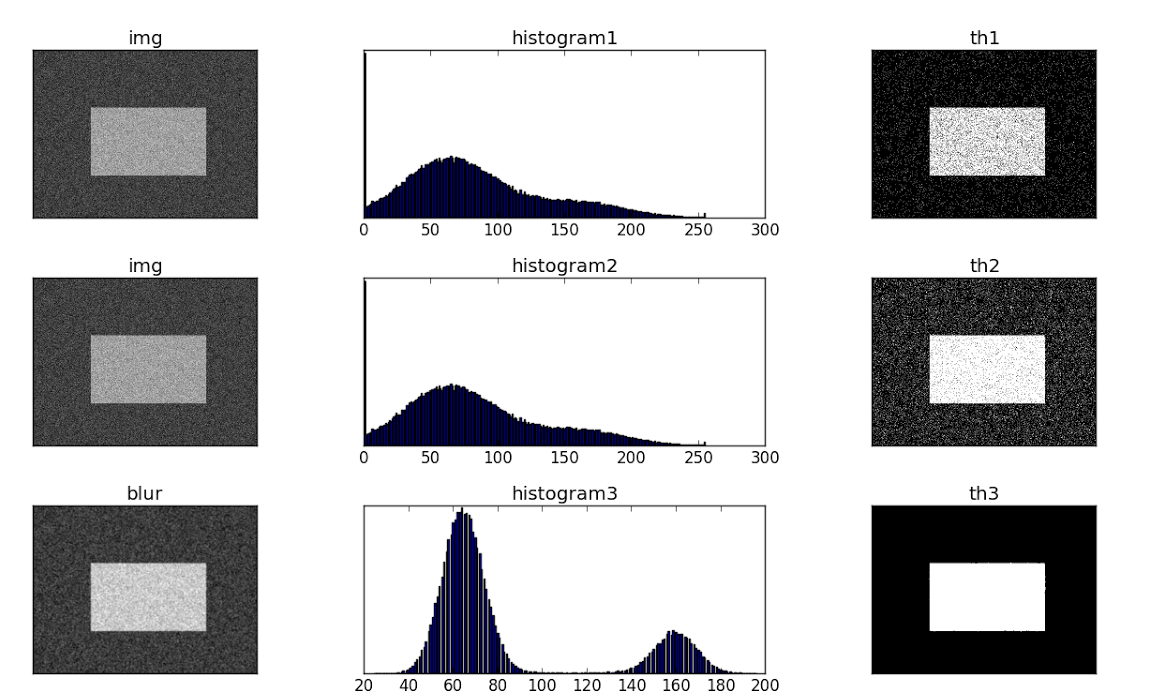
\includegraphics[width=0.8\textwidth]{otsuthres}
    \label{fig:threshold}
    \caption{Verschiedene Schwellwertverfahren im Vergleich \cite{Opencv:2013}}
\end{figure}

Reihe 1 zeigt dabei eine Schwellwertfunktion mit dem globalen Schwellwert $v=127$, in Reihe 2 wurde 
der Schwellwert mit dem Verfahren von Otsu bestimmt. In Reihe 3 wurde das Eingabebild zuerst mit einem 
Gaußfilter geglättet und weichgezeichnet, wie es auch bei der Zozosuit-Messfunktion benutzt wird. In Abbildung 
\ref{fig:thres_zozo} werden die einzelnen Bearbeitungsschritte eines Bildabschnittes mit Zozosuit veranschaulicht.


\begin{figure}[H]
    \centering
    \subfigure[Basis]{
\includegraphics[width=0.45\textwidth]{im_base}}\qquad 
    \subfigure[Graustufen]{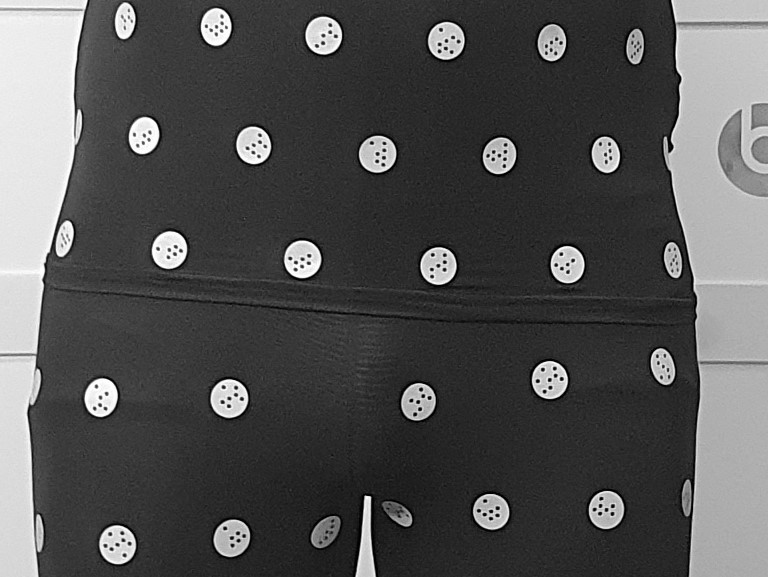
\includegraphics[width=0.45\textwidth]{im_gray}}\qquad 
    \subfigure[Gaußfilter]{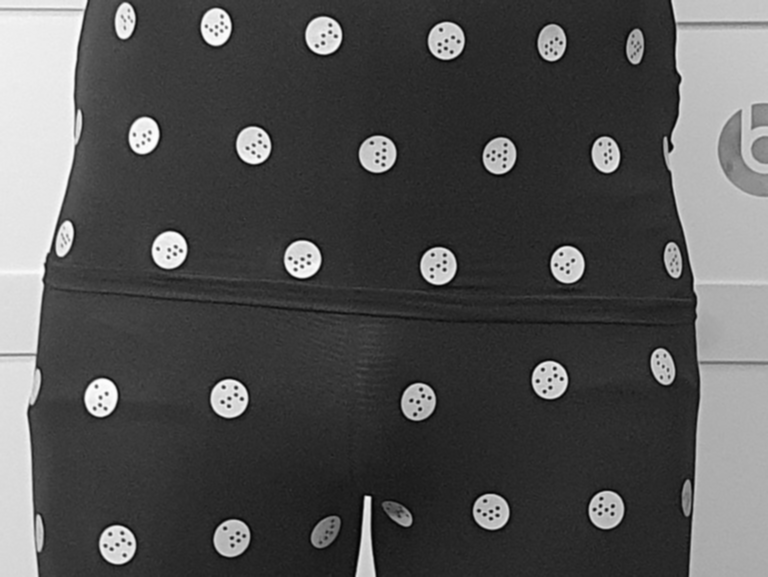
\includegraphics[width=0.45\textwidth]{im_blur}}\qquad 
    \subfigure[Schwellwert]{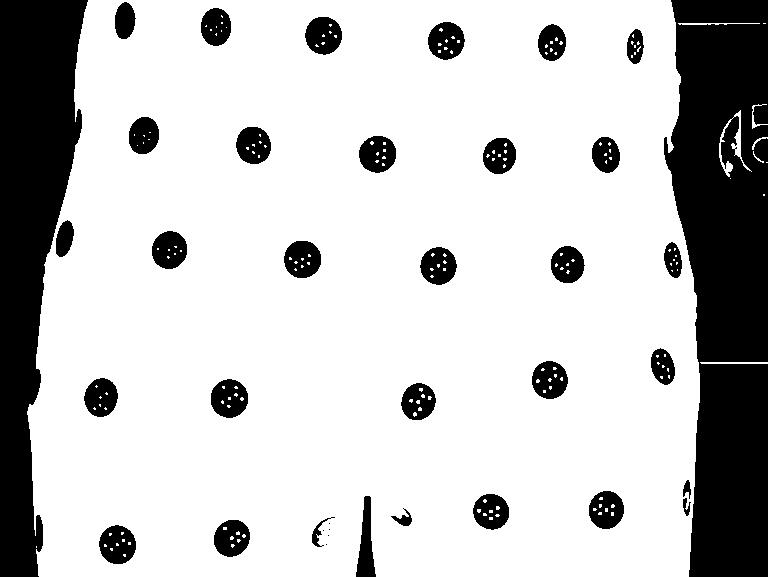
\includegraphics[width=0.45\textwidth]{im_threshold}}
    \label{fig:thres_zozo}
    \caption{Image-Pipeline bei der Aufbearbeitung des Basisbildes mit der Zozosuit-Messfunktion}
\end{figure}

Aus dem aufgearbeiteten, binären Bild werden in einem weiteren Schritt durch die OpenCV-Funktion \texttt{findContours(\dots)} die Konturen
der Messpunkte ausgelesen. Unter einer Kontur bersteht man eine Kurve, die alle Punkte entlang einer Begrenzung verbindet, welche die gleiche 
Farbe oder Itensität haben. \texttt{findContours(\dots)} gibt eine Liste von Konturen zurück, die allerdings nicht nur Messpunkte des Zozosuits
umfasst, sondern auch ungewollte Konuren. Dementsprechend müssen ungewollte Konturen gefiltert werden. Vorerst erfolgt die Entfernung
aller Konturen, die nicht in etwa zu der Größe der Messpunkte mit einem Durchmesser von 2 Centimetern passen. Konturen, die weder rund noch elliptisch sind,
können ebensfalls aussortiert werden. Da weitere Verarbeitung mit sehr flachen Ellipsen fehleranfällig ist, werden elliptische Konturen,
bei denene das Verhältnis von kürzestem Durchmesser zu längstem Durchmesser kleiner als $\frac{1}{10}$ ist, ebenfalls aussortiert. In einem
letzten Schritt erfolgt die Transformation der Elipsen zu kreisen, da diese einfacher zu verarbeiten sind. Die Transformationsmatrix wird
mit der OpenCV-Funktion \texttt{getAffineTransform(\dots)} mit drei Punkten auf berechnet, dem Mittelpunkt, dem kurzen Scheitelpunkt sowie dem langen
Scheitelpunkt. Nach der Transformation der Konturen mit der entsprechenden Transformationsmatrix ergibt sich eine Menge an Bildern der kreisförmigen Messpunkte 
des Zozosuits.

\section{Punkt auf Zozosuit}

Für die Ermittlung der einzigartigen ID eines Messpunktes ist dessen Aufbau wichtig, welcher im folgenden beschrieben wird.
Ein Messpunkt hat einen Durchmesser von 2 Centimetern, zudem existieren Messpunkte an Hals und Füßen, die nur einen Durchmesser
von einem Centimeter haben, da diese jedoch keine ID haben, spielen sie hier keine Rolle. In jedem der circa 300 Messpunkten befindet
sich eine Anordnung von 4 bis 10 kleinen Pünktchen mit einem Durchmesser von 2 Millimeter, welche eine einzigartige ID wie folgt widerspiegeln, sowie ein
Pünktchen im Mittelpunkt.
\begin{figure}[t]
    \centering
    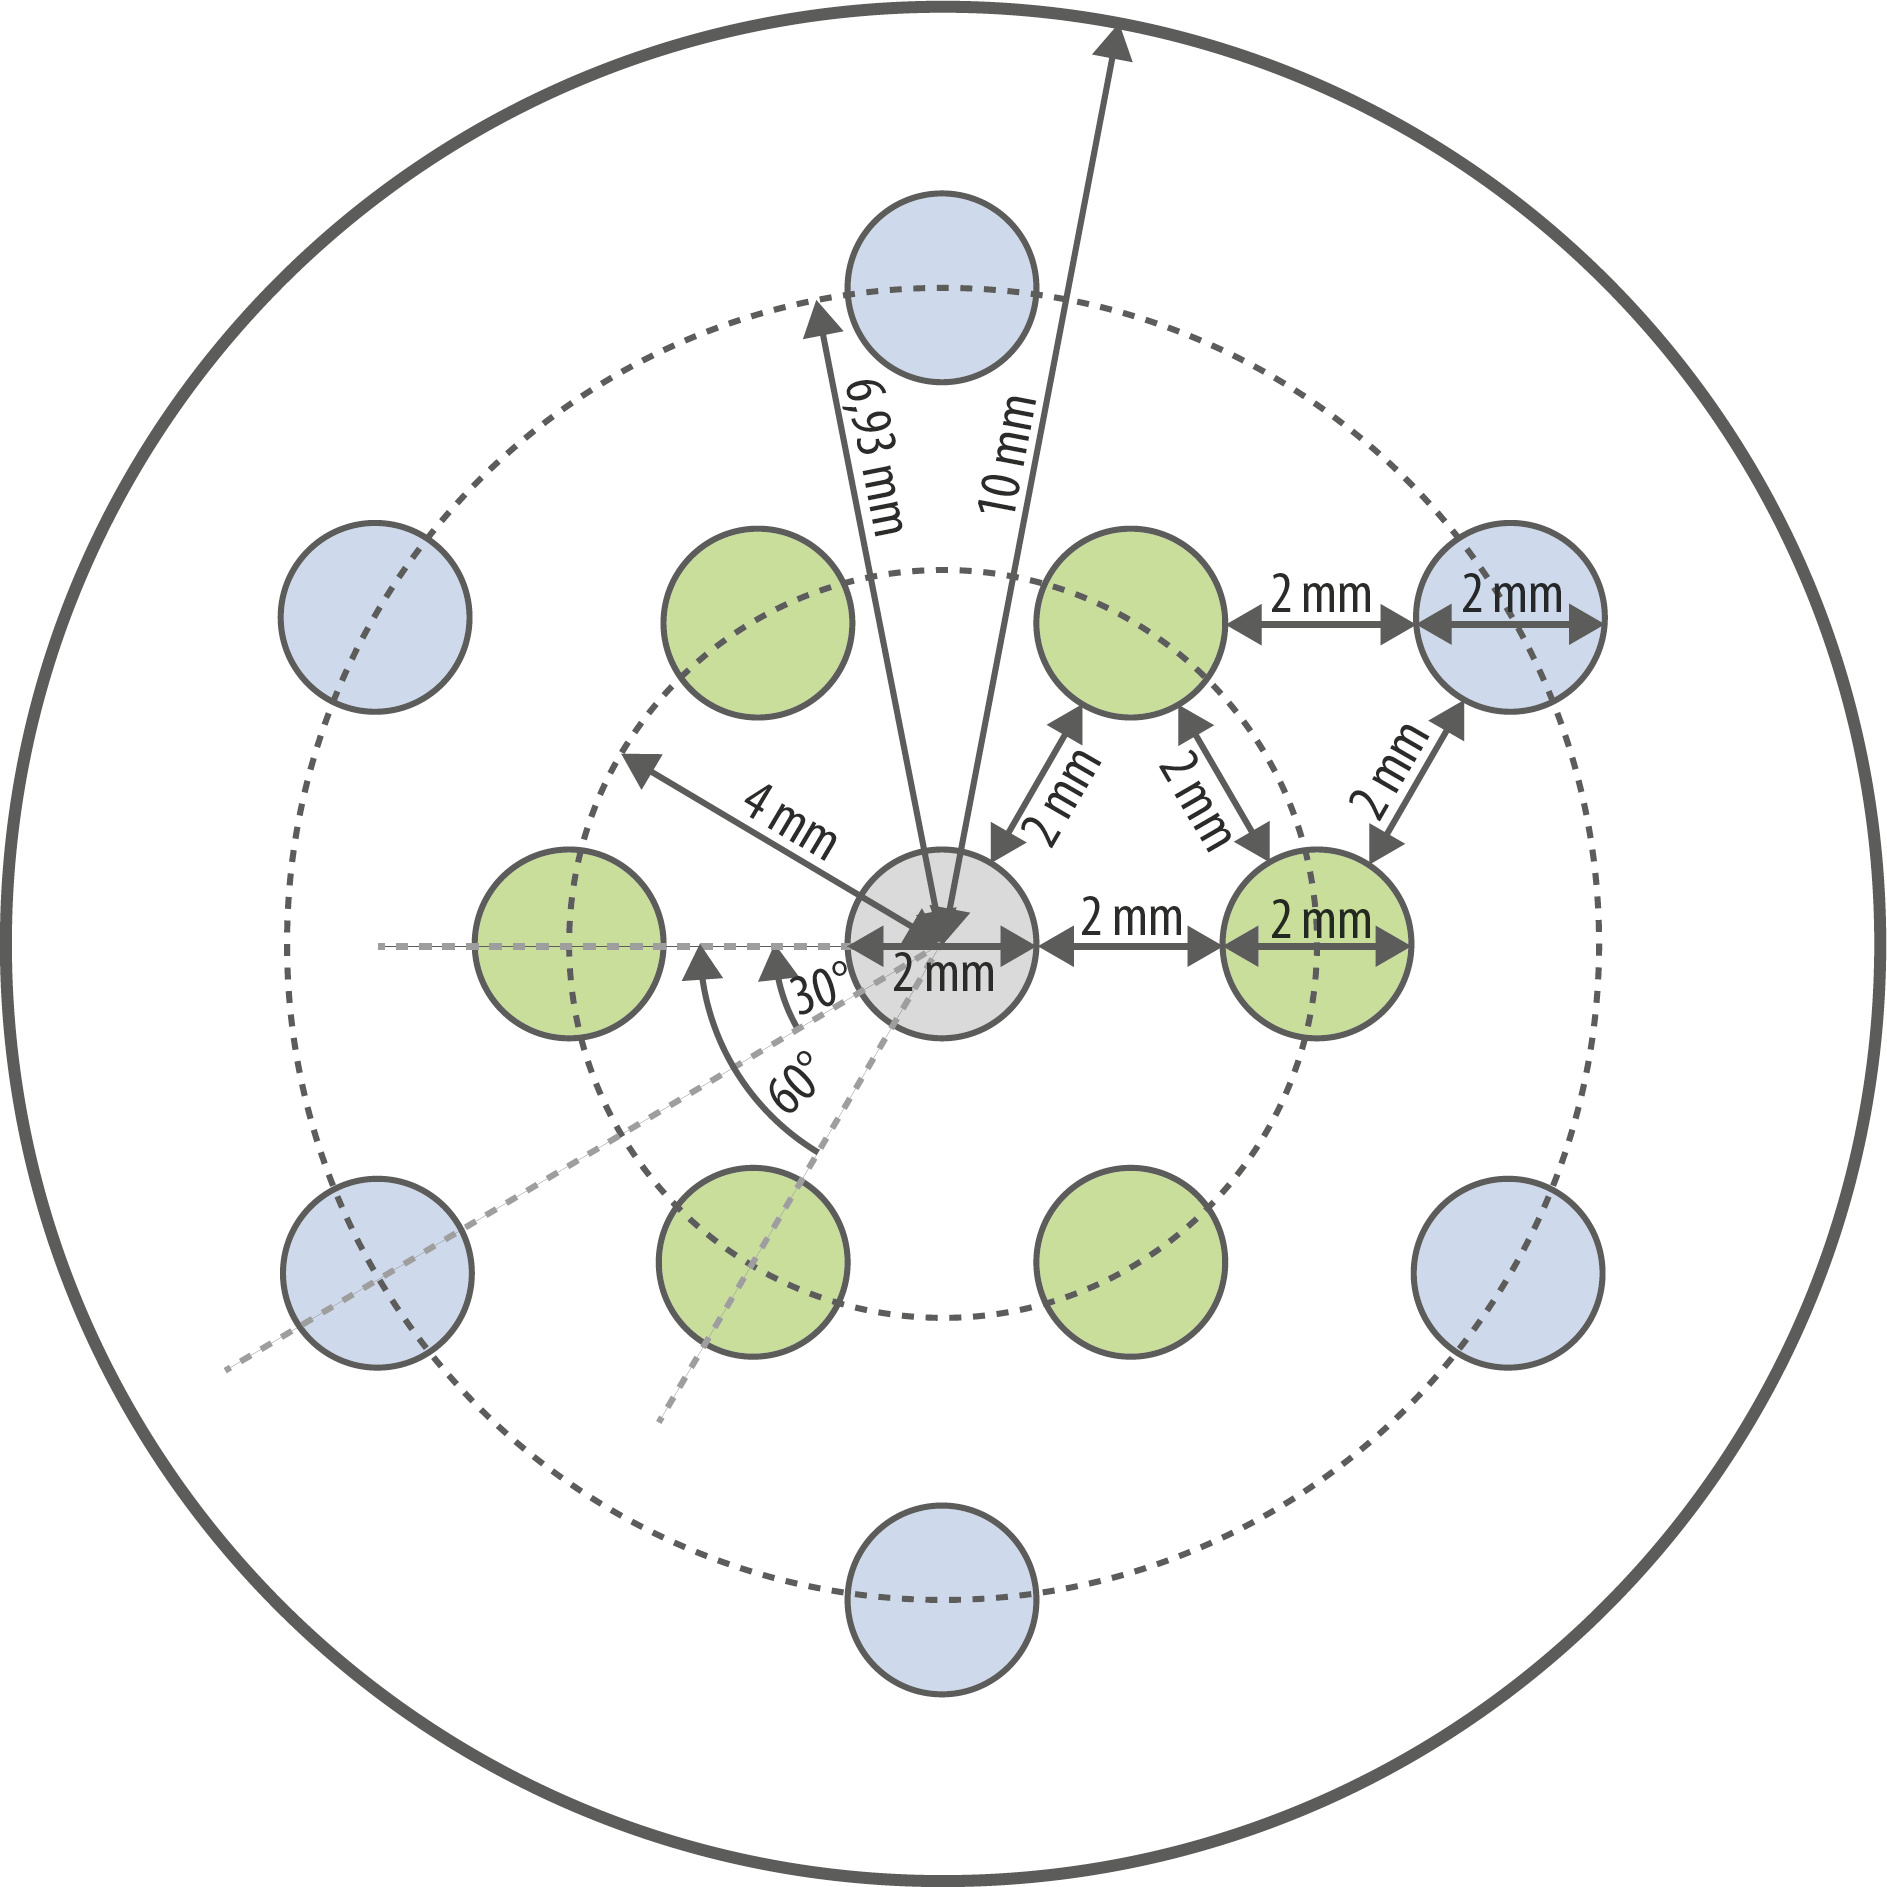
\includegraphics[width=0.9\textwidth]{Zozopunkt}
    \label{fig:zozopunnkt}
    \caption{Aufbau eines Messpunktes des Zozosuits \cite{Pina:2018}}
\end{figure}
In einem Messpunkt befinden sich je 6 mögliche Positionen für Pünktchen auf einem Kreis mit dem Radius von 4 Millimeter und einem Winkel von 60° zum 
Nachbarn. Weitere 6 mögliche Positionen befinden sich auf einem Kreis mit dem Radius von etwa 6.93 Millimetern, ebenfalls mit einem WInkel von 60° zudem
Nachbarn, allerdings um 30° zu jenen Positionen im inneren Kreis (vgl. Abb. \ref{fig:zozopunnkt}).

So ergeben sich insgesamt 12 mögliche Positionen für Pünktchen, welche je ein Bit kodieren. Existiert ein Pünktchen auf einer Position,
ist der Bitwert 1, ansonsten. Dies ergibt eine $2^12=4096$ möglichen Punkteanordnungen. Die Pünktchen des äußeren Kreises kodieren im
Uhrzeigsinn gehend, beginnend beim Pünktchen im Norden, die ersten 6 Bits. D Pünktchen im inneren Kreis stellen im Uhrzeigersinn gehen, angefangen
beim Pünktchen um 30° im Uhrzeigsinn verschoben zum Norden, die zweiten 6 Bit dar. Allerdings müssen sich bei jedem Messpunkt 
sowohl auf dem inneren Kreis als auch dem 
äußeren Kreis mindesten 2 und maximal 5 Pünktchen befinden. Da die Messpunkte in der Wirklichkeit (um 60°,120°,180°,240°,300°) verdreht sein können, werden zudem nur jene der
6 möglichen Punkteanordnung gezählt, deren 12 Bit die höchste Zahl kodieren. Diese beiden Einschränkungen ergeben eine Anzahl von 608 einzigartigen
IDs für die 2 Centimeter großen Messpunkte. \cite{Pina:2018}

\section{Erkennung der ID}

Für die Erkennung der ID eines Messpunktes auf dem Zozosuit muss dieser zuerst in eine Position gedreht werden, sodass die Positionen
der Pünktchen mit jene in Abbildung \ref{fig:zozopunnkt} übereinstimmen. Hierbei wird eine Maske mit den 12 möglichen Punktepositionen
erzeugt über dem Messpunkt erzeugt und 60 Mal um 1° verschoben. Ist diese Maske so gedreht wie die tatsächlich vorhandenen Pünktchen 
im Messpunkt, haben die maskierten Pixel eine kleinere durchschnittliche Helligkeit als alle Masken mit abweichendem Winkel. 
Mit dem nun richtig gedrehten Messpunkt kann die ID ermittelt werden. Hier werden 12 Masken, die je eine der 12 Punkteposition freistellen,
über den Messpunkt gelegt. Liegt der durchschnittliche Farbwert der so freigestellten Punkteposition über dem Mittelwert von 127, wird davon ausgeganen,
dass sich auf dem Messpunkt an dieser Stelle ein Pünktchen befindet, was als binäre 1 interpretiert wird. Liegt der durchschnittliche Farbwert
unter dem Mittelwert von 127, befindet sich an dieser Stelle kein Pünktchen und der binäre Wert wird auf 0 gesetzt. Dieser Vorgang wird 12 Mal wiederholt,
sodass jeder Punktepositionen ein binärer Wert zugewiesen wird. \cite{Pina:2018}

Zusammengesetzt ergibt sich dadurch eine 12-Bit ID. Da jedoch 5 weitere mögliche Ausrichtungen des Punktes möglich sind, und die IDs 
konsistent sein sollen, wird wie im letzten Kapitel beschrieben immer nur die höchst mögliche ID der 6 verschiedenen Drehungen der Punkteanordnung
verwendet. Hierbei wird 6 Mal je auf die ersten und letzten 6 Bit ein Bitshift nach links durchgeführt, das 1. Bit an die 7. Position kopiert und
und das 1. Bit gelöscht. Der höchste enstehende binäre Werte ist die ID des Punktes. \cite{Pina:2018}
\chapter{Stand der Technik}
\label{ch:sdt}

\section{Frontend}

In dieser Studienarbeit sollen Bilder von einer Person im ZOZOSUIT gemacht werden und diese anschließend ausgewertet und als 3D-Modell dargestellt werden. Da sowohl Bilder 
gemacht, als auch Grafiken angezeigt werden, bietet sich das Smartphone als Frontend an. 

In Deutschland besitzen 81\% der Bevökerung ab 14 Jahren ein Smartphone, in jungen Altersgruppen steigt der Prozentsatz auf über 95\% \cite{misc:marktforschung_smartphone}. 
Für Smartphones bestehen zwei dominante Betriebssysteme: Android und i\acrshort{os}. Mit einem Marktanteil von 69,8\% ist Android in Deutschland Marktführer für 
Smartphonebetriebssysteme, gefolgt von i\acrshort{os} mit 29,8\%. Andere Betriebssysteme, wie Windows und Blackberry, 
besitzen einen Marktanteil von 0,4\%. \cite{misc:kantarworldpanel}. \newline
Für Android entwickelte Apps basieren auf Java oder Kotlin, während i\acrshort{os}-Apps in Swift oder Objective-C entwickelt werden. Des Weiteren gibt es Tools und \glspl{sdk}, 
mit welchen Apps entwickelt werden können, welche mit wenigen Einschränkungen auf beiden Betriebssystemen lauffähig sind:
\begin{itemize}
    \item \textbf{React Native}: React Native ist ein JavaScript Framework, welches die \gls{ui} in native (Android oder iOS spezifische) Elemente umwandelt. Die Logik bleibt dabei unverändert. Das Framework wird von Facebook, Instagram und Uber benutzt.
    \item \textbf{Xamarin}: Xamarin ermöglicht es Entwicklern eine gemeinsame Logik für Android und iOS zu schreiben. Die jeweilige UI wird allerdings in einer nativen Programmiersprache entwickelt.
    \item \textbf{Flutter}: Flutter ist ein \gls{sdk}, welches von Google erstellt, und im Jahr 2018 erstmals in der Version 1.0 veröffentlicht wurde. Das \gls{sdk} verwendet die, ebenso von Google entwickelte, Programmiersprache Dart. Flutter ermöglicht es UI-Komponenten zu entwickeln, welche auf beiden Betriebssystemen konsistent sind.
\end{itemize}

Damit Apps im App Store von Apple veröffentlicht werden dürfen, benötigt der/die Entwickler/-in eine Mitgliedschaft im Apple Developer Program. Diese kostet pro Jahr 99 US-Dollar \cite{misc:appledeveloper}.
Des Weiteren kann eine für i\gls{os} entwickelte Anwendung nur in einer Apple-Umgebung (Macbook, \dots) kompiliert werden. \newline
Aus diesen Gründen, und wegen dem Verbreitungsanteil von 29,8\% in Deutschland, ist das Entwickeln dieser App für eine reine i\gls{os}-Umgebung nicht sinnvoll. \newline

Um Apps im Google Play Store zu veröffentlichen, wird eine einmalige Registrierungsgebühr von 25 US-Dollar benötigt \cite{misc:androiddeveloper}. Eine jährliche Gebühr ist 
nicht vorhanden.

React Native ermöglicht zwar das Entwickeln einer Anwendung für iOS und Android, jedoch werden nicht alle plattformspezifischen \glspl{api} unterstützt. Nicht unterstützte 
\glspl{api} müssen in der nativen Programmiersprache erstellt werden. Es muss somit trotzdem für iOS und Android separat entwickelt werden. \cite{misc:reactnative_vs_native}\newline
Die nicht vollständige Unterstützung nativer \glspl{api} ist eine Schwachpunkt aller Frameworks, welche das gleichzeitige Entwickeln für iOS und Android ermöglichen. \newline
Xamarin bietet durch die Unterstützung von .Net und Microsoft Visual Studio die beste Entwicklungsumgebung. Jedoch mindert die geringe Popularität die verfügbaren Hilfestellungen 
durch andere Entwickler/-innen \cite{misc:flutter_reactnative_xamarin}. \newline
Laut einer Umfrage von Stack Overflow ist Flutter das beliebteste der drei vorgestellten Frameworks \cite{misc:so_popularity}. Es ist jedoch auch das jüngste 
(Version 1.0 im Jahr 2018) und kann somit auf den geringsten Anteil an verfügbaren Hilfestellungen zurückgreifen. Auch die Unterstützung durch Bibliotheken von Dritten ist 
noch nicht so ausgereift, wie bei den anderen Frameworks. Allerdings steht eine gute Online-Dokumentation zur Verfügung, welche unter \cite{misc:flutter_docs} erreichbar ist.
\cite{misc:flutter_reactnative_xamarin}

Ein weiterer negativer Aspekt der Cross-Platform-Entwicklung sind Systemupdates von iOS oder Android. Ein Systemupdate kann neue Funktionen hinzufügen und alte Verändern 
oder Entfernen. Während bei nativen Plattformen darauf geachtet wird, dass alle Änderungen rückwärtskompatibel sind, müssen sich Cross-Platform-Frameworks erst an die 
Änderungen anpassen. Dadurch kann es während Übergangsphasen zu fehlerhaftem Verhalten der App kommen.

In Anbetracht dieser Punkte ist das Entwickeln des Frontends als reine Android-App oder als plattformübergreifende App unter Verwendung eines Frameworks denkbar. Die Wahl fällt hierbei
auf eine Cross-Platform-App, welche mithilfe von Flutter, und der damit verbundenen Programmiersprache Dart, erstellt wird. Dies begründet sich darin, dass bei einer reinen Android-
Anwendung knapp ein Drittel der Smartphonebesitzer keinen Zugriff auf die App haben würden. Die Wahl von Flutter ergibt sich aus der guten Online-Dokumentation und der Popularität, 
durch welche möglicherweise auftretende Probleme besser gelöst werden können. \newline
Als Entwicklungsumgebung wird Android Studio gewählt, da dieses ein Flutter-Plugin besitzt und einen 
Emulator bereitstellt, mit welchem verschieden Smartphones auf verschiedenen \acrshort{api}-Stufen simuliert werden können.
\chapter{Zusammenfassung und Ausblick}

klappt zwar mit suit, geht aber theoretisch bessre ohne, zozosuit2 könnte das vermutlich aber schaffen   % Zusammenfassung
\appendix
\chapter[Anhang]{}
\label{ch:anhang}

                     % Anhang

\printbibliography                          % Literaturverzeichnis
\end{document}